\chapter{緒言} \label{chp:1}

\section{研究背景}
	\subsection{サービスロボット}
	総務省平成30年版情報通信白書\cite{ServiceRobot-ref1}によると，日本の労働人口が減少していくと予測されている．それにより，今後多くの企業において人材不足が加速すると予想される．特に大きく影響を受ける労働集約型の農林水産業や建設業，運輸・流通業やサービス業においては，既に経営課題として顕在化している．日本銀行が発表している全国企業短期経済観測調査（短観）の業種別計数によると，2014年以降は全ての業種において人手は「不足」となっており，特に建設業や運輸業，対事業者サービス業，対個人サービス業において深刻であることがわかる(図\ref{fig:noPeople})．\cite{ServiceRobot-ref1}
	\begin{figure}[h]
		\centering
		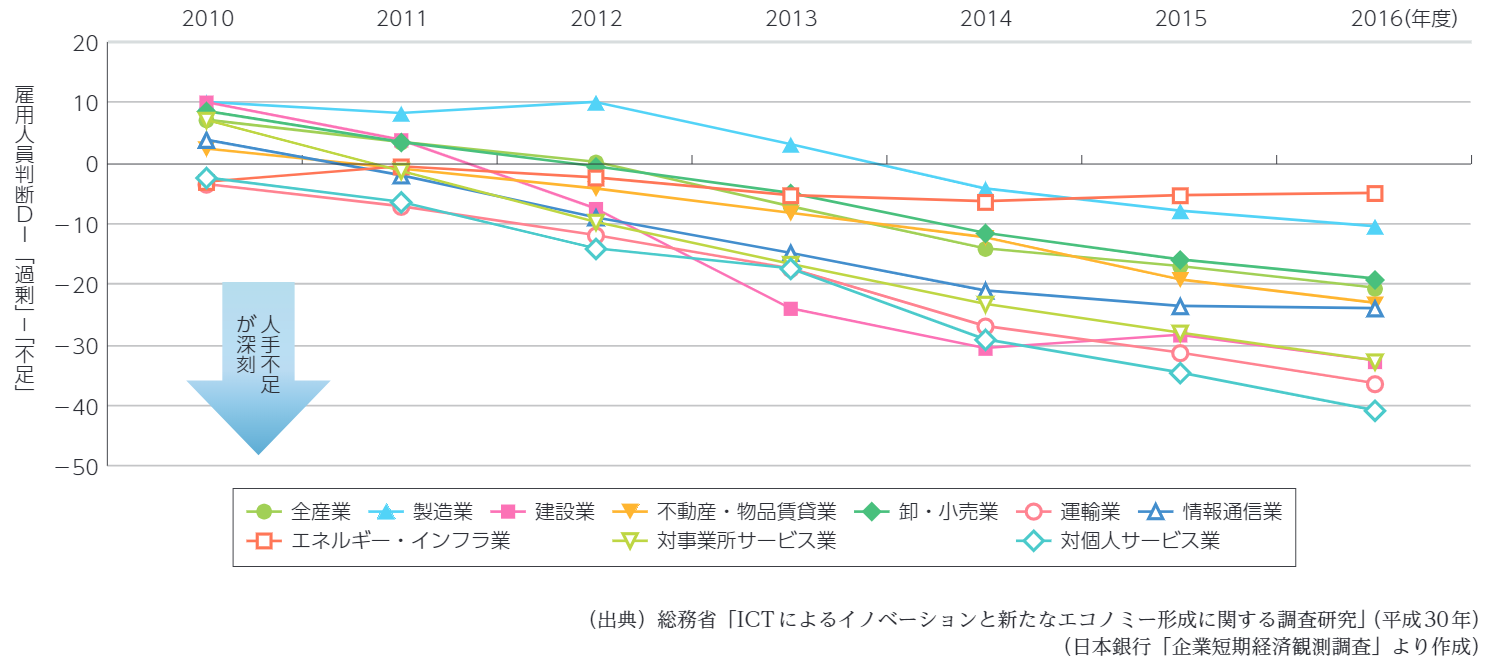
\includegraphics[width=1\linewidth]{fig/chp1/noPeople}
		\caption{業種別の雇用人員判断DI（「過剰」－「不足」）}
		\label{fig:noPeople}
	\end{figure}

	また，総務省平成30年版情報通信白書\cite{ServiceRobot-ref1}により，労働人口が減少する影響で物流，ヘルスケア・介護，外食，店舗といった製造業以外のサービスロボットの市場規模は，負担の軽減等を目的として拡大が続いている．物流での箱詰めやピッキング等でサービスロボットの活用が広がっているほか，店舗の接客やホテルの受付・クローク業務等一般消費者と直接的に接するサービスロボットの活用も増加している．\cite{ServiceRobot-ref1}(図\ref{fig:ServiceRobot})．
	\begin{figure}[h]
		\centering
		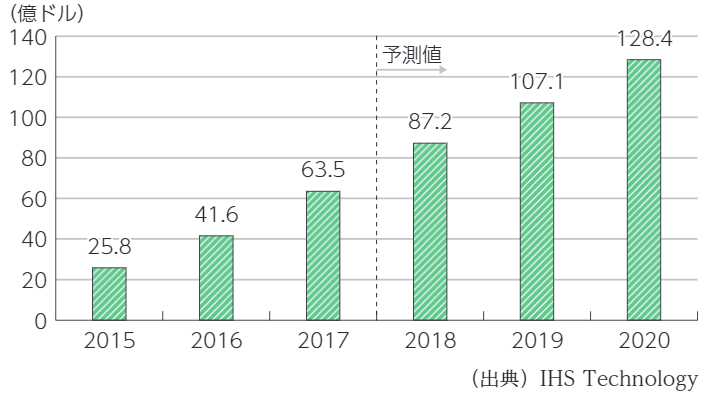
\includegraphics[width=1\linewidth]{fig/chp1/ServiceRobot}
		\caption{世界のサービスロボット市場規模の推移及び予測}
		\label{fig:ServiceRobot}
	\end{figure}

	更に，2020年オリンピックは東京で開催するため，翻訳や案内のような対個人サービスの需要が拡大すると予想される．

	\subsection{料理ロボット}
	料理作業は人間にとって非常に重要な作業である．
	料理ロボットは人間を支援するサービスロボットの研究の一分野として，世界中で研究が盛んである．	
	
	\subsection{注ぎ作業}
	料理作業において，注ぎ作業は高い頻度で現れる．
	例えば，液体調味料(酢や醤油など)を入れる作業や料理に水を加える作業などが挙げられる．
	注ぎ作業は単なる注ぎ先の容器に注ぐだけではなく，料理のレシピに示された分量の通り定量的に注ぐ必要がある．
	定量的でないと，料理の味あるいは食感が変わってしまう．

\section{関連研究と考察}\label{sec:Intro}
	\subsection{注ぎ作業}
	ロボットによる注ぎ作業の研究はこれまでにも行われている．
	Schenckら\cite{Related1}によるRGB-D画像と熱画像を用いたお湯の注ぎ作業，
	Kennedyら\cite{Related2}による数学的モデルを用いた定量的な注ぎ作業，
	Mottaghiら\cite{Related4}によるCNNを用いた画像中の容器の容積や液体の体積の推定，
	Gravotら\cite{Related3}らによる料理作業のプランニングとシミュレーションなどがあげられる．
	我々の研究グループも，計量スプーンを用いた調味料の計量作業\cite{福島さんの修論}を実現している．
	
	液体を定量的に注ぐとき，人間であれば計量カップや計量スプーンあるいは秤を使って決められた量の液体を容器に注ぐ．
	しかし，このような道具を使う方法では正確な分量を計量できる反面，計量作業を別途しなければならない問題がある．
	例えば，水をいくつかのコップに均等に分ける場合，容器ごとに水の体積を量る必要があるため，計量作業に時間がかかる．
	ロボットによる作業の場合，計量カップなどを用いなくても，カメラ等を用いて容器の形状を計測することによって注がれた液体の体積を計算することが出来るため，計量作業をする手間を減らすことが可能になる．
	
\section{研究目的}\label{sec:purpose}
以上の考察を踏まえ，本研究の目的は計量器具を使わずに行う双腕ロボットによる定量的な注ぎ作業の実現である．
その目的を実現するためにはまず以下の2つの課題を解決することが必要である．

%\begin{enumerate}
%	\item 注いだ体積の測定．\label{enum:main-purpose1}
%	\item 注ぎ動作の制御．\label{enum:main-purpose2}
%\end{enumerate}

\begin{description}
  \item[1] 注いだ体積の測定．\label{enum:main-purpose1}
  \item[2] 注ぎ動作の制御．\label{enum:main-purpose2}
\end{description}

%\ref{enum:main-purpose1}
\par1について，注いだ体積が分からないなら，「定量的」とは言えない．
したがって，注いだ体積の測定はこの研究の中心であり，できるだけ容器の形や姿勢に縛られない，汎用性が高い方法が求められる．

%\ref{enum:main-purpose2}
\par2について，注いだ体積がわかったとしても，注ぎ動作の制御が高精度に行えないと，液体がこぼれたり一気に大量の液体が流入する可能性がある．
これは誤差となるため，注ぎ作業を実行している時においては，注ぐ容器の回転角度の制御が重要である．

しかし，上記2つの課題を解決するだけでは定量的な注ぎ作業を実現させることはできない．
それ以外に解決すべき課題が以下の３つである．
具体的には：
%\begin{enumerate}
%	\item 容器の認識．	\label{enum:sub-purpose1}
%	\item 容器モデルの取得．\label{enum:sub-purpose2}
%	\item 容器を掴む動作の作成．	\label{enum:sub-purpose3}
%\end{enumerate}

\begin{description}
  \item[3] 容器の認識．	\label{enum:sub-purpose1}
  \item[4] 容器モデルの取得．\label{enum:sub-purpose2}
  \item[5] 容器を掴む動作の作成．	\label{enum:sub-purpose3}
\end{description}

%\ref{enum:sub-purpose1}
\par3について，容器の認識は更に2つの課題に分けられる．
第1に容器が置かれている位置の検出をする必要がある．
容器の位置が分からなければ他の課題(例えば，モデルの取得や容器を掴むことなど)が実現できない．
第2に注ぐ容器と注ぎ先容器を判断する必要がある．
どちらが注ぐ容器かが分からない場合，注ぎ作業を進めることはできない．

%\ref{enum:sub-purpose2}
\par4について，容器モデルの形式(関数で表すモデルや点群など)や容器モデルの取得する手段である．
本論文が使用した方法は容器モデルが必要なため，容器モデルがないと実行できない点に注意する必要がある．

%\ref{enum:sub-purpose3}
\par5について，各種の容器に対して，適切な掴み方や掴む所を選択することである．
注ぎ動作を制御するため，ロボットアームは必ず道具を使用し，容器を掴み，計算した姿勢に容器を移動や回転を行う．
容器を掴めないと，計算した姿勢に移動できず，注ぎ動作が失敗する．

上述の課題を実現することで，目標体積に液体を容器に定量的に注ぐことを目指す．

\section{研究概要}
本研究は以下の２つのことを実現した．
\begin{enumerate}
	\item テーブル上の注ぐ容器と注ぎ先の容器を識別し，注ぐ容器を掴み，注ぎ先の容器に指定した目標体積の液体を入れること．
	\item テーブル上の注ぐ容器の外側の形状と容器中の液体の体積を検出し，注いだ体積と注ぐ容器の傾き角度の関係を求め，注ぎ先の容器に指定した目標体積の液体を入れること．
\end{enumerate}
		
\section{論文構成}
本論文の構成は次の通りである．
第2章は注ぎ作業を実現するための検討と注ぎ作業の手法を説明する．第3章は実験のためのロボットシステムについて説明する．第4章は2章で提案した手法の実装である．第5章は提案した手法を検証するための実験である．第6章は本研究のまとめと今後の課題を述べる．
	
	
	
	
	